\section{吉布斯采样}
\label{sec:17.4}

到目前为止,本章已经介绍了如何通过迭代更新$x\rightarrow x' \sim T (x'|x) $在概率分布$q(x)$上采样的方法.
但是,还没有说明怎样确保$q(x)$是有效的概率分布.
本书主要考虑两种基本方法.第一种方法根据给定的通过学习得到的$p_{model}$推导出$T$,下文将会详细介绍从EBMs(energy-based model)采样的例子.
第二种方法是直接参数化$T$并学习,使其平稳分布可以隐式地定义$p_{model}$的兴趣点.
第二种方法的例子将在章节"\textcolor{red}{20.12}"和"\textcolor{red}{20.13}"阐述.

在深度学习中,通常使用马尔科夫链从以基于能量的模型定义的概率分布$p_{model}$中采样.
此例中,马尔科夫链所需的$q(x)$就是$p_{model}$.
为得到满足需求的$q(x)$,必须选择合适的$T(x'|x)$.

为了构建马尔科夫链,一种概念上简单有效的方法就是使用\textit{吉布斯采样}从$p_{model}$中采样.
在吉布斯采样中,通过选择一个变量$x_i$实现从$T(x'|x)$中采样,$x_i$的选择方法取决于它在基于能量模型结构的无向图$\mathcal{G}$上的邻居变量.
只要给定的所有邻居节点都条件独立,也可以同时对多个变量采样.
在16.7.1中的RBM(受限玻尔兹曼机)例子中,RBM的所有隐含层单元可以被同时采样,是因为他们都条件独立于其他的给定可视层单元.
同样的,因为对于给定的隐含层单元,所有的可视层单元都是条件独立的,因此所有的可视层单元也可以同时被采样.
以这种方式同时更新多个变量的吉布斯采样方法,被称为块吉布斯(block gibbs)采样.

从$p_{model}$中采样来设计马尔科夫链的代替方法是可行的.例如,Metropolis-Hastings算法就广泛应用于其他学科领域.
在深度学习领域实现无向建模,除吉布斯采样外很少使用其他方法.
改进采样技术是一个潜在的研究领域.

\section{分离状态混合的挑战}
\label{sec:17.5}

$MCMC$方法的主要问题是混合效果比较差.理想情况下,从$P(x)$分布设计的马尔科夫链中得到连续采样之间将会是完全相互独立的,
这些采样在$x$空间下访问不同的区域可能性与他们的概率成正比.
然而,尤其是在高维情况下,MCMC样本之间会强相关.
我们称这种行为是缓慢混合,甚至是失败混合.
相对于链(随机变量被采样)的状态,$MCMC$方法的缓慢混合可以被看作是在能量函数上随意地执行了类似嘈杂梯度下降(noisy gradient descent)操作,
或者等效地在概率函数上执行嘈杂爬山(noisy hill climbing)操作.
马尔科夫链往往使用渐进策略(在马尔科夫链状态空间中),从组态$x_{(t-1)}$到$x_{(t)}$,
能量$E(x_{(t)})$往往低于或约等于能量$E(x_{(t-1)})$,偏好会产生较低能量组态的移动.
当从相对不可能的组态(比来自$p(x)$的典型构型具有更高的能量)开始时,链趋向于逐步降低能量的状态仅仅偶尔移动到另一种状态.
一旦链找到了低能量的区域(例如,假设变量是图片中的像素点,则低能量的区域可以是同一对象的图像中的连通的多边形),我们称其之为一个状态,链将会尝试在状态上游走(类似于随机游走).
一旦跳出那个状态,一般会返回原状态或者(如果找到了逃离路线)会移动到另一个状态.
问题是成功的逃离路线很少有很多有趣的分布,所以马尔科夫链将会在同一状态而不是它应有的状态上连续采样.

在使用吉布斯采样算法时这一点是显而易见的$(Sec. 17.4)$.
在这种情况下,在特定的步骤内从一个状态转移到邻近状态的概率取决于状态之间"能量势垒"(energy barrier)的形状.
被高能量势垒(低概率区域)分隔的两个状态之间是不太可能发生转移的(在能量势垒的高度方面).
如图$17.1$所示.
当多个高概率状态被低概率区域分隔时会出现问题,特别是当吉布斯采样每步仅仅更新一小部分变量,而这部分变量的值主要由其它变量确定时.

举个简单的例子,假设基于能量模型的两个变量$a$和$b$,他们是带符号的二进制,取值为-1和1.
对于模型$E(a,b)=-wab$,如果$w$是一个大正数,那么这个模型中的$a$和$b$极有可能具有相同的符号.
如果使用$a=1$的吉布斯采样步骤来更新$b$,那么$b$的条件分布则是由$P(b=1|a=1)=\sigma(w)$确定的.
如果$w$很大,$b$也赋值为1的概率接近于1.
同理,如果$a=-1$,则将$b$赋值为-1的概率接近1.
根据$P_{model}(a,b)$模型,两个变量的符号可能相同.
也就是说,吉布斯采样不会改变变量的符号.

实际应用场景更具有挑战性,因为不仅要关注两个状态之间的转移,而且在更具一般性的真实模型中可能更关心多个状态之间的转移.因为状态混合困难性,获取覆盖大多数状态的可靠样本集合花费的代价巨大,而且到达马尔科夫链稳定分布状态的收敛速度非常慢等诸多原因,这样的多个状态之间的转移是很难的.

有时这个问题可以通过找到含有高度依赖性单元的群体并按块同时更新所有这些单元来解决.
然而不幸的是,这种依赖性是复杂的,从这样的群体中采样是难以计算的.
毕竟,马尔科夫链最初被引入来解决的问题就是怎样从一组变量中采样.

\begin{figure}[htbp]
	\centering
	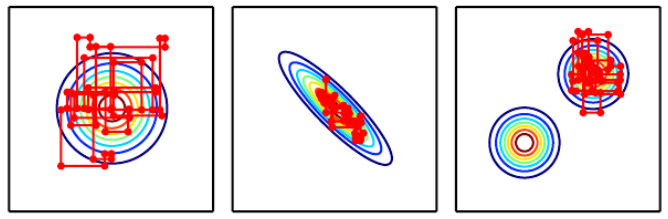
\includegraphics[width=5in]{fig/chap17/chap17.1.png}
	\caption{三种分布的吉布斯采样路径,在这两种情况下,马尔科夫链以同样的模式初始化.
	$($左图$)$两个条件独立变量的多变量正态分布.因为变量之间是条件独立的,所以吉布斯采样混合的很好.
	$($中图$)$变量高度相关的多变量正态分布.变量之间的相关性使得马尔科夫链很难混合.因为每个变量的更新都要取决于其他变量,相关性降低了马尔科夫链从起始点移动到其他状态的概率.
	$($右图$)$广泛分离模式的高斯分布的混合是非轴对称的.因为当一次仅改变一个变量时,马尔科夫链难以改变状态,所以吉布斯采样混合的很慢.}
	\label{fig:chap17.1.png}
\end{figure}

在含有隐含变量的模型中,定义了联合分布$p_{model}(x|h)$,常常通过交替在$p_{model}(x|h)$和$p_{model}(h|x)$中对$x$进行采样.
从快速混合的目的出发,我们希望$p_{model}(h|x)$有更高的熵.
但是,从学习到有用的$h$的表达式的目的出发,我们又希望$h$有足够的信息来编码并重建$x$,这意味着$h$和$x$应该有很高的交互信息.
这个两个目标是相互矛盾的.
常见的生成模型可以非常精确地将$x$编码为$h$,但是往往不能混合地很好.
这种情况在玻尔兹曼机中很常见-玻尔兹曼机学习到的分布越尖锐,马尔科夫链从分布模型中的采样就越难以混合良好.
这个问题在图$17.2$中说明.

当兴趣分布具有多种结构且每一类有单独的样本,所有上述问题都可能导致$MCMC$方法在兴趣分布上失效:
概率分布集中在许多状态周围,这些状态被高能量区域分隔开.
这类分布就是我们在许多分类问题中期望的,状态之间的较差混合导致$MCMC$方法收敛地非常缓慢.

\begin{figure}[htbp]
	\centering
	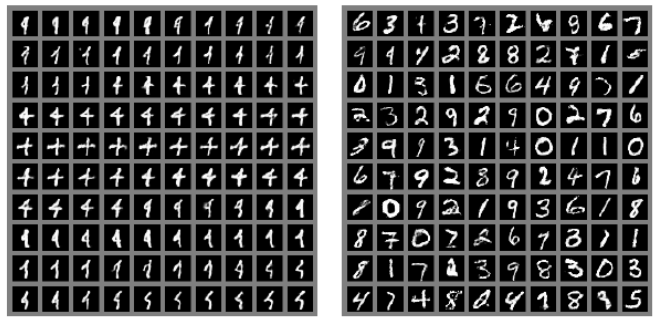
\includegraphics[width=5in]{fig/chap17/chap17.2.png}
	\caption{在深度概率模型中漫混合问题的例子.每个图像应该从左到右,从上到下阅读.
	$($左图$)$是来自吉布斯采样的连续样本应用于MNIST数据集上训练的深度玻尔兹曼机.连续样本之间是很相似的.
	因为吉布斯采样是在深度图模型中执行的,所以这种相似性更多地基于语义而不是原始视觉特征,
	但是吉布斯链仍然难以从分布的一种状态转换到另一种状态,例如通过改变数字标识.
	$($右图$)$是来自生成对抗网络的连续祖代样本.因为祖代采样独立于其他样本而生成每个样本,所以没有混合问题.}
	\label{fig:chap17.2.png}
\end{figure}

\section{17.5.1 基于回火的状态混合}
\label{sec:17.5.1}

当一个分布显示出的形态是低概率区域围绕着高概率的“尖峰”时候,这个分布的不同状态很难混合。很多快速混合技术都基于构建的可以替代目标分布的版本,在新构建的分布中峰没有目标分布高,周围的谷也没有目标分布低。基于能量的模型提供了一个特别简单的方法来实现。到目前为止,我们已经描述了一个基于能量的模型来作为概率分布的定义,如下式:
$p(x)\propto exp(-E(x))$                   (17.25)
基于能量的模型可以增加一个额外的参数$\beta$来控制这个分布快速达到峰值。
$p_{\beta}(x)\propto exp(-\beta E(x))$              (17.26)
参数$\beta$通常被描述为温度的倒数,这反映了基于能量的模型在统计物理学中的起源。当温度下降到零并且$\beta$趋于无穷大时,基于能量的模型变得稳定。当温度趋于无穷大并且$\beta$下降到零时,离散$x$的分布变得均匀。

通常来说,可以训练一个模型来得到$\beta=1$时的估计值。然而,我们可以使用其他温度,特别是$\beta<1$处的温度。回火是通过描绘$\beta<1$的采样来实现$p_{1}$的多个状态之间快速混合的一个一般性策略。

为了混合不同的模式,基于回火转换的马尔可夫链(Neal在1994年提出)暂时从更高的温度分布采样,然后再恢复到从单位温度分布上采样。
这些技术已经被应用到一些模型上,比如RBMs(Salakhutdinov在2010年提出)。
另一种方法是使用并行回火(Iba在2001年提出),其中马尔可夫链在不同温度下,并行模拟了许多不同的状态。
最高温度状态下混合缓慢,但是最低温度状态在温度为1时提供了来自模型的精确样本。
转换操作包括在两种不同温度水平下随机切换状态,因此从高温时隙中获得的一个高概率样本可以跳到一个较低温度的时隙中。
这个方法也被应用到RBMs中(Desjardins等在2010年提出;Cho等在2010年提出)。
虽然回火是一种很有使用前景的方法,但是现在研究人员还没能在从复杂EBMs采样的问题上取得突破性进展。
一个可能的原因是为了使得回火有效临界温度周围的温度转换必须是非常缓慢的(因为温度是逐渐降低的)。

\section{17.5.2 深度会促进混合}
\label{sec:17.5.2}

当从一个隐变量模型$p(h,x)$采样时,我们看到,如果$p(h|x)$对$x$编码太长,则从$p(x|h)$采样时$x$变化很小并且混合效果差。
解决这个问题的一个方法是,将$h$作为一个深度表示,在这个深度表示中,将x编码到h中来使得在$h$区间中的马尔科夫链更容易混合。
许多表征学习算法,如自动编码器和$RBMs$,更容易产生一个在$h$上的边缘分布,其比在$x$上的原始数据分布更统一和更单调。
可以说这是由于在使用所有存在的表征空间来试图最小化重建误差时,因为不同的训练样本在$h$区间上更容易划区分,在训练样本上最小化重建误差将实现的更好,并因此获得更好的相互独立性。
Bengio等人(2013a)观察到,在顶层h区间上,正则化过的自动编码器或$RBMs$的深栈堆产生边缘分布,其出现更加广阔和均匀,对于不同模式之间具有较小的间隙(在实验中)。
在较高层的空间中训练$RBM$可以使Gibbs采样在模式之间更快地混合。
然而,它仍然不清楚如何利用这种观察以便更好地训练和从深度生成模型中抽样。

尽管混合比较困难,但蒙特卡洛方法是有效的并且经常被认为是可用的最好的工具。
实际上,它是用于面对无向模型的难处理配分函数的主要工具,将在接下来进行讨论。
